\documentclass[MS]{dukedissertation}

%%%%%%%%%%%%%%
% temp additions for notes
\usepackage{todonotes}
\usepackage[top=1.5cm, bottom=1.5cm, outer=5cm, inner=2cm, heightrounded, marginparwidth=3.5cm, marginparsep=1cm]{geometry}
%%%%%%%%%%%%%%



\usepackage{fontspec}
\defaultfontfeatures{Numbers=OldStyle}
\setmainfont{Minion Pro}


\usepackage{amsmath, amssymb, amsfonts, amsthm}
\usepackage{graphicx}
\usepackage{natbib}
\usepackage{url}
\usepackage{color}
\usepackage{bm}
\usepackage{subfigure}
\usepackage{graphicx}
\usepackage{mathabx}
\usepackage{multirow}
\usepackage{setspace}
\usepackage{booktabs}
\usepackage{adjustbox}

\renewcommand{\bibname}{References}
\graphicspath{{./Pictures/}}

\author{Amogh Uday Karnik}
\title{Design and Usability Testing of a Mobile Phone-Based Patient Management System for Women in Rural Kenya}
\supervisor{Eric Green}
\department{Duke Global Health Institute}


\date{2014} % Year

% Copyright text.  If undefined, default is 'All rights reserved'
% (Example sets the text to a hyperlinked Creative Commons Licence)
\copyrighttext{ All rights reserved except the rights granted by the\\
   \href{http://creativecommons.org/licenses/by-nc/3.0/us/}
        {Creative Commons Attribution-Noncommercial Licence}
}

% Committee Members other than supervisor.  No more than five beyond the supervisor allowed.
\member{Nimmi Ramanujan}
\member{Lavanya Vasudevan}

\usepackage[xetex,bookmarks=true,colorlinks, linkcolor=black,urlcolor=black,citecolor=black, linktoc=section,]{hyperref}


\begin{document}

%-----------------------------------------------------------------------------%
%Title Page
%-----------------------------------------------------------------------------%
\maketitle

%-----------------------------------------------------------------------------%
%Abstract
%-----------------------------------------------------------------------------%
\abstract

\paragraph{Each year, more than 300,000 of women die from complications related to pregnancy, childbirth, or abortion. At least eighty percent of these deaths can be prevented by a set of proven interventions provided by a skilled practitioner, and two-thirds of all infant deaths can be prevented with antenatal care provided by a health professional during the first six weeks after delivery. However, delays in recognizing the need to seek care, delays in reaching health care facilities, and delays in receiving adequate care can all make delivery of the aforementioned interventions extremely challenging. Baby Monitor -  a novel, mobile-phone based screening system – hopes to help pregnant women and new mothers overcome these barriers to accessing care. In its current iteration, women listen to pre- and post-natal screening questions in their local language and respond by pressing keys on their mobile phones. The proposed research will focus on expanding the scope of this service by using the screening information to send patients health information, make referrals to local health facilities based on patient needs, and dispatch community health workers for targeted home visits. The development and testing of these features will ultimately lead to a system that helps address the delays in receiving effective in maternal and child health care and complements the existing health care system in Kenya.}} %Path to abstract.tex

%-----------------------------------------------------------------------------%
%Frontmatter: Table of Contents, List of Tables, List of Figures, List of Abbreviations
%-----------------------------------------------------------------------------%
\tableofcontents % Automatically generated
\listoftables	% If you have any tables, automatically generated
\listoffigures	% If you have any figures, automatically generated
%\abbreviations

% You can put here what you like, but here's an example
%Note the use of starred section commands here to produce proper division
%headers without bad '0.1' numbers or entries into the Table of Contents.
%Using the {\verb \begin{symbollist} } environment ensures that entries are
%properly spaced.

%\section*{Symbols}
%
%Put general notes about symbol usage in text here.  Notice this text is
%double-spaced, as required.
%
%\begin{symbollist}
%	\item[$\mathbb{X}$] A blackboard bold $X$.  Neat.
%	% Optional item argument makes the symbol/abbr
%	\item[$\mathcal{X}$] A caligraphic $X$.  Neat.
%	\item[$\mathfrak{X}$] A fraktur $X$.  Neat.
%	\item[$\mathbf{X}$] A boldface $X$.
%	\item[$\mathsf{X}$] A sans-serif $X$. Bad notation.
%	\item[$\mathrm{X}$] A roman $X$.
%\end{symbollist}
%
%\section*{Abbreviations}
%
%Long lines in the \texttt{symbollist} environment are single spaced, like in
%the other front matter tables.

\begin{symbollist}
	\item[CHV] Community health volunteer
	\item[CHEW] Community health extension worker
	\item[IVR] Interactive voice response
	\item[MAMA] Mobile Alliance for Maternal Action
	\item[mHealth] Mobile health
	\item[m-Pesa] Mobile money service utilized in Kenya
	\item[SMS] Short message service, used interchangeably with text messaging service
	\item[VoIP] Voice over Internet Protocol
\end{symbollist}
} % List of Abbreviations. Start file with '\abbreviations'

%-----------------------------------------------------------------------------%
% ACKNOWLEDGEMENTS -- included file should start with '\acknowledgements'
%-----------------------------------------------------------------------------%
%\include{{./Acknowledgements/acknowledgements}}

%=======================================%
% MAIN BODY OF PAPER
%=======================================%

%-----------------------------------------------------------------------------%
% Chapter 1: Overview
%-----------------------------------------------------------------------------%
\chapter{Chapter One}
\section{Introduction}
\subsection{Maternal Mortality}
\paragraph{Every day, approximately 800 women die of complications related to pregnancy, childbirth, or abortion around the world. According to the World Health Organization (WHO), an estimated 287,000 maternal deaths occcurred in 2010 alone \citep{WHO2012}. Most maternal deaths occur between the third trimester and the first six weeks after delivery - the majority of which occur either during or within the first few days after delivery \citep{WHO2012}. The most common causes of maternal death during this period are severe bleeding, hypertensive disease, and infection \citep{WHO2012}. Moreover, the burden of maternal mortality is greatest among developing countries where most low-income women deliver in their own homes. In sub-Saharan Africa, one in every sixteen women will die of pregnancy-related causes - a lifetime risk higher than anywhere else in the world \citep{Ronsmans2006}.}

\paragraph{Most maternal deaths are avoidable. At least 80\% of maternal deaths can be prevented by a set of proven interventions provided by a skilled practitioner. Two-thirds of all infant deaths can be prevented with postnatal care provided by a health practitioner during the first six weeks after birth. However, delays in recognizing the need to seek care, accessing health care facilities, and receiving  adequate care make the delivery of the aforementioned interventions extremely challenging \citep{Thaddeus1994}. }

\paragraph{These three delays have disproportionately affected women and families living in rural and remote regions. High costs of care, far distances between villages and health facilities, and relative lack of skilled practitioners in these regions all contribute to lower prenatal care coverage and deliveries at health facilities among women in rural areas. Thus, pregnancy-related complications such as anemia or infection, which would normally be identified early on during the course of a pregnancy, commonly go unnoticed. These complications, when not addressed, can prove to be deadly for both mother and child during the critical days during and after delivery.}

\paragraph{Community-based interventions have emerged as potentially effective methods in reducing the delays associated with maternal mortality. Since gaps exist between the community and the health facility, whether due to costs, distance, or other factors, the common theme among community-based strategies has been to extend provision of care into villages and individual households. In recent years, some of the most promising of these community-based interventions for maternal and child health have focused on using mobile phones.}

\paragraph{Over the past decade, mobile phones have had an incredible impact on low to middle income countries. Mobile phone technology has enabled millions of people to communicate to and from some of the most poor and remote areas of the world - especially in sub-Saharan Africa \citep{Adler2007}. Moreover, increased phone penetration has allowed mobile providers to expand the roles of mobile phones  beyond that of simple communication devices.}

\paragraph{In 2007, Safaricom - the largest mobile provider in Kenya - launched a mobile phone-based payment service called m-Pesa. Designed for the ''unbanked'', m-Pesa allowed users to make deposits and withdrawals, transfer and receive money to and from others, pay bills, and purchase airtime through a simple interface accessible on all mobile phones. This service was rapidly adopted, with 20,000 users registering for m-Pesa accounts within a month of its launch \citep{Hughes2007}. As of 2010, m-Pesa has been adopted by 9 million users, roughly 40\% of Kenya's adult population \citep{Mas2010}. This model of mobile banking has been replicated in a number of developing countries, including Uganda, Tanzania, and India.}

\paragraph{The success of m-Pesa and other mobile payment systems set a precedent for the use of mobile phone technology in developing countries. As mobile phone penetration has continued to increase, mobile phone technology has been applied in a variety of contexts in the health care space. These applications have largely aimed to address gaps and challenges that exist within health systems in developing countries \citep{Labrique2013}. The earliest of these interventions involved using mobile phones as a primary method of data collection, allowing health workers to report data immediately at the point of care. This strategy has been used to implement mobile-phone based vital registration systems (such as Uganda Mobile VRS) and establish electronic health record systems(such as OpenMRS), both of which rely on data entry at the point of care and allow for data collection in rural or remote areas \citep{Labrique2013}.}

\paragraph{Many mobile phone-based interventions have focused on using text messaging, due to its availability, low cost, and instantaneous nature.  Previous literature has focused on using text messages as reminders for patients and evaluating their utility for improving care seeking behaviors \citep{ColeLewis2010} and clinical attendance \citep{Guy2012}. Additional studies have evaluated the utility of text message reminders for improving adherence to treatment regimens for HIV \citep{Horvath2012} and self-management of diabetes care \citep{Krishna2008}. Each of these studies concluded that text messaging interventions can have a positive impact on health behaviors and outcomes.}

\paragraph{While the majority of mHealth interventions have focused on text-based interactions through mobile phones, relatively few have relied on voice-based interactions. Though text messages are inexpensive and instantaneous in nature, voice-based applications offer an avenue to overcome potential literacy barriers that may be present in many developing countries. Interactive Voice Response (IVR) is a method by which users listen to recorded messages and report information using their phone's touch-tone keypad. IVR systems have  previously been implemented to assist in the treatment of chronic patients suffering from heart failure, diabetes, and mental health illnesses \citep{Piette2000}. In these cases, patients used IVR to report information remotely, rather than reporting information via a clinical interview. Patients were found to be more willing to report concerns through the IVR system than in person with a provider \citep{Piette2000}. Previous literature has also suggested that IVR could be used for educational purposes for both patients and health care providers \citep{Labrique2013, Lee2003}.}

\paragraph{Over the past decade, mHealth technologies have been widely implemented in the field of maternal and child health. Specifically, mHealth programs have been used to expand data collections to reach financially and geographically isolated populations, provide support and information for providers at the point of care, improve response to obstetric emergencies, and promote healthy behaviors among pregnant women and new mothers \citep{Tamrat2012}.}

\paragraph{Many of these interventions have used text-based interactions as the primary mode of interacting with both providers and patients. For example, text messages have been used to train and educate midwives about safe delivery and postnatal care practices in South Africa \citep{Woods2012}. Text message reminders have also been used to improve timeliness of routine visits by community health workers in Tanzania \citep{DeRenzi2012}. The Mobile Alliance for Maternal Action (MAMA) has created a package of text messages that provide educational information to pregnant women and new mothers throughout their pregnancies and one year post-delivery \citep{MAMA}. Interventions centered around MAMA messages have been implemented in several developing countries, including South Africa, India, and Bangladesh. In each of these countries, MAMA messages were adapted for each region based onthe known cultural norms and beliefs regarding pregnancy and child care \citep{McCartney2012}. These programs may also help improve the overall patient experience for pregnant women who have opted to receive prenatal care. Studies have shown that pregnant women who received biweekly text messages offering support during the time between prenatal care visits had higher satisfaction levels with their care than women who did not receive any messages \citep{Jareethum2008}.}

\paragraph{Compared to text message-based interventions, relatively few mHealth programs have focused on using voice-based interaction. These programs have primarily focused on using voice-based applications to engage with community level providers, rather than patients. The Obstetric Helpline program in Rajastan, India has enabled community members and health workers to connect patients to the appropriate health facilities during emergencies, thereby attempting to reduce the delays associated with seeking and receiving care \citep{UNICEF2008}.  The Healthline Project, a speech-based IVR system currently in development in Pakistan, has attempted to improve access to information for community health workers at the point of care \citep{Sherwani2007}.}

% Work in description of MoTECH program: text and IVR system designed for midwives to use in Ghana.%


\paragraph{Although the established literature has provided examples of various programs with promising elements, there is a need for an mHealth program that integrates voice and text interfaces to engage with both patients and providers in the maternal and child health space. In 2012, principal investigator Eric Green and his research team at the Population Council began development and testing of a new mHealth service called Baby Monitor. In the pilot phase of this project, the Baby Monitor team partnered with InSTEDD, a non-profit technology group, and Jacaranda Health, a non-profit maternity clinic in Nairobi, to develop and refine a health screening system that reaches pregnant women directly through their mobile phones via IVR. Participants completed automated screening calls and identical, follow-up clinical screenings with a nurse at Jacaranda Health at several points before and after delivery. Calls were scheduled based on the WHO guidelines for focused prenatal care and the Kenyan Ministry of Health's guidelines for postnatal immunizations. The results of this pilot phase have yet to be published, but the mobile screens were found to be reliable when compared to the in person follow-up assessments. Moreover, uptake for the service was high and women reported that they enjoyed receiving calls from the Baby Monitor system.}

\paragraph{This project was built upon the existing Baby Monitor framework and aimed to develop a comprehensive, voice and text based system that would supplement the patient-centered screening service.\todo{Justify why this study was focused on referrals and patient management. Conclude with objective(s) of the study. -A}}
% Needs work %%%


\section{Fieldwork Site}
\subsection{Maternal Mortality in Kenya}
\paragraph{Maternal mortality is a very serious public health problem in Kenya. According to the 2008-09 Kenya Demographic and Health Survey (DHS), the maternal mortality rate was estimated to be 488 per 100,000 live births - a figure among the highest in the world \citep{DHS2010}. Much of this burden of mortality can be attributed to lack of early detection of pregnancy-related complications. Nationwide, 47 percent of women attend four or more prenatal care visits, and 44 percent of women living in rural areas attend four or more prenatal visits \citep{DHS2010}. To make matters worse, most women do not receive prenatal care in the early stages of their pregnancies, as 15\% of all Kenyan women make their first prenatal visit during the first trimester \citep{DHS2010}.}

\paragraph{Also contributing to the burden of maternal mortality in Kenya is the relatively high proportion of women who choose to deliver in their homes. According to DHS data, an estimated 56\% of births in Kenya take place in the home, while 43\% of births take place in a health facility. This trend is even more pronounced in rural areas, where 63\% of women choose to deliver at home compared to only 35\% in a health facility \citep{DHS2010}.}

\paragraph{It is not surprising that prenatal care coverage and place of delivery are closely related. According to DHS data, 87.5\% of women who did not attend any prenatal care visits delivered at home, with approximately 10.7\% delivering at either a public or private health facility. Meanwhile, 38.4\% of women who attended at least four prenatal care visits chose to deliver at home, with 60.3\% opting to deliver in a public or private health facility. Thus, women who receive prenatal care are more likely to deliver at a health facility.}

\paragraph{In an effort to improve upon these issues, the Kenyan Ministry of Health declared that all maternal health services would be free of charge for all women at all public health facilities in the country \citep{MOH2013}. According to this policy, all women visiting any type of public health facility would be entitled to free prenatal, delivery, and post-delivery care. While this policy would remove a major financial barrier that prevents women from visiting facilities in many remote and rural areas of the country, it remains to be seen how effective or sustainable it will be moving forward.}

\subsection{Kenyan Health System}
\paragraph{Kenya is divided into 47 counties, each of which is comprised of a number of divisions. Each of these divisions is subdivided into numerous individual community units. The current health system is divided into four tiers that reflect these geographic divisions: national referral hospitals, county hospitals, primary care services, and community level services. \citep{SPA2010}}

\paragraph{Health care delivery at the level of the community unit is the foundation of this system. According to the Community Strategy guidelines published by the Kenyan Ministry of Health in 2006, community level care should be focused on prevention of infectious diseases, control of noncommunicable diseases, maternal and child health services, family planning activities, and effective sanitation and hygiene practices \citep{CommunityStrategy2006}. Providers at this level are the community  health volunteers (CHVs), who opt to serve their communities on a voluntary basis. Identified and selected by their fellow community members, CHVs are the primary interface between individuals and the public health system. According to the Ministry of Health guidelines released in 2006, each CHV should be responsible for 20 households or 100 individuals \citep{CommunityStrategy2006}. Community health extension workers (CHEWs) are responsible for training and supervising a cadre of 25 CHVs each. In a single community unit, 2 CHEWs should supervise approximately 50 CHVs in order to provide care to 5,000 people \citep{CommunityStrategy2006}. Typically, CHEWs are based out of the local dispensary, collecting information from CHVs and visiting their assigned community units on a regular basis.}

\paragraph{Dispensaries and clinics serve clusters of community units. These facilities aim to provide both preventative and curative services, including prenatal care, family planning, and basic emergency care. Some of these facilities may also be equipped to handle deliveries. Providers at this level of care include nurses, and clinical officers.  These facilities are by far the most widespread across the country, with 2,413 government-funded dispensaries and clinics in operation as of 2010. \citep{SPA2010}}

\paragraph{Hospitals at the county level provide both inpatient and outpatient care, including comprehensive maternity and emergency care. Most patients at these hospitals have been referred from dispensaries or clinics from communities within the county. Providers at this level of care include nurses, midwives, clinical officers, and doctors. There were 225 government-funded primary hospitals at the coutny level as of 2010. \citep{SPA2010}}

\paragraph{National referral hospitals - such as Kenyatta National Hospital in Nairobi and Moi Teaching and Referral Hospital in Eldoret -  provide the most sophisticated level of care within the Kenyan health system. Most patients at these hospitals have been referred from primary or secondary hospitals at the county level. Providers found at this level of care include nurses, clinical officers, doctors, and many other specialized healthcare personnel. \citep{SPA2010}}

\paragraph{This study was conducted in the Ndivisi Division of Bungoma County, a rural region approximately 60km west of Eldoret. 
Ndivisi, which has a population of 77,599, is divided into 11 community units \citep{Census2009}. The research site was comprised of two community units, Sinoko and Sitabicha, with a combined population of 10,744 \citep{Census2009}. These two community units were local to Sinoko clinic, the largest clinic in Ndivisi division. Sinoko is one of only three health facilities in the area with the personnel, equipment, and supplies to handle deliveries on a regular basis. The two remaining facilities are located in Webuye town, which is approximately 16km away from the clinic.}

\paragraph{At the time of the study, there were 55 CHVs and 3 CHEWs working in the study catchment area. On average, each CHV was responsible for approximately 195 individuals and 36 households - far more than the 100 individuals and 20 households suggested by the Ministry of Health's Community Strategy guidelines. Most individual villages in the study community units only had one CHV assigned to provide services.}


\section{Research Methods}
\todo{This section isn't finished yet. Will be adding more detail on HCD methodology and how it specifically relates to the project. I think more detail on methodology is OK in this Chapter, but less is probably better in the Journal Article section. What do you think? - A}

\paragraph{The overall objective of this study was to develop a system that could fill existing gaps and fit within the current health infrastructure in Kenya. Ideally, this system would leverage text and voice interactions to better connect patients, CHVs, and clinic nurses so as to improve care-seeking behaviors and overall delivery of maternal and child health care. In order to build such a system, the research team adopted a human-centered design framework. Within this framework, the users of the system are targeted from the beginning of the research process. Throughout the design and development phases, the users are regularly consulted in order to ensure that the end product meets their unique needs and priorities.}

Methods for this study were adopted from the Human-Centered Design Toolkit, a collection of strategies and techniques focused on developing solutions that meet the needs of users in the developing world \citep{HCDToolkit}. This toolkit defined three iterative phases of the human-centered design process: Hear, Create, and Deliver. 

\subsection{Hear Phase}
The Hear phase is primarily focused on understanding the users, their tasks, and their environment. This is accomplished through a number of methods aimed at collecting users' stories, observations, and insights regarding the use. In this case, the users of the patient management service were identified as the CHVs, given their foundational role in the health system. Additionally, nurses were also identified as key informants for the Hear phase, given their role in providing maternal and child health services at the dispensary, clinic, and hospital level. 

The methods employed during this phase included a focus group discussion with CHVs, shadow days with CHVs, and a focus group discussion with the clinic nurses. The focus group discussion with the CHVs was loosely structured, with the research team asking a series of open-ended questions regarding CHV roles, responsibilities, and work flow related to maternal and child health. CHVs were asked to expand on topics such as data collection and patient referral within the discussion as well. Following this focus group discussion, the research team shadowed two of the CHVs participating in the focus group on two separate occasions. This allowed for a better understanding of the CHVs' daily responsibilities and experiences conducting home visits within their village. It also gave the CHVs an opportunity to describe some of the challenges that they face in visiting homes, collecting information, and managing care for the entirety of their village. The final aspect of the Hear phase was a focus group discussion with nurses staffed at the study clinic. Similarly, the discussion was facilitated by the research team and focused on the nurses' experiences working with pregnant women and new mothers with emphasis on patient referral. This allowed for a better understanding of the referral process from the clinic side, and gave the nurses a chance to voice their concerns, frustrations, and suggestions for improving the methods by which CHVs and nurses convey information to one another. Using these findings, the research team was able to identify a set of themes and design principles that would govern the development process going forward. 

\subsection{Create Phase}
The Create phase is centered around producing a design solution based on the results of the Hear phase. In this case, the goal of this phase was to develop a prototype system that engaged CHVs through IVR and text messages and complemented their daily tasks and responsibilities. 

The prototype system integrated several technologies: Verboice, a platform for designing and initiating phone calls over the internet, a Voice over Internet Protocol (VoIP) provider in Kenya, a software framework called Asterisk that connected Verboice to the VoIP provider, a telecommunications company in Kenya that delivered the calls to the mobile phones of users, and an SMS gateway provider that sent text messages to the users' mobile phones. An analysis engine, written in R, integrated each of these technologies to trigger new calls through Verboice, trigger text messages through the SMS gateway provider, and process call data. This analysis engine was responsible for ensuring interoperability between each of the individual components, allowing information to be collected from through IVR and be transmitted back to CHVs via text message. 

\subsubsection{Verboice}

Verboice is an open source, web-based platform for creating projects that interact with users through IVR. This platform allows users to listen to audio messages in multiple languages, respond to questions with their touch-tone keypads, and record their own voice messages. Verboice was used to create a series of call flows designed to collect information from CHVs about home visits or deliveries that they would like to report. Each call flow was designed with the same basic framework. First, the user calls into the Baby Monitor system and immediately hangs up - a process known as `''flashing'' a number. This is a common practice in Kenya, especially when a mobile phone user does not wish to be charged for an incoming call. After the user flashes the Baby Monitor number, the user receives a free incoming call through Verboice. During this call, the user listens to a series of instructions and questions that addressed the design themes and principles identified during the Hear phase. For questions that required a 'yes' or 'no' answer, users were asked to press '1' or '3' on their keypads, respectively. For other questions, users were asked to enter numerical data through their keypads. No data or answers to questions were stored locally on their phones; all responses were stored securely in a database connected to the research team's Verboice account. 

\subsubsection{SMS Gateway}
The research team also created a set of text messages specific to the roles and responsibilities of the CHVs in order to supplement the IVR system. These messages were designed to use information provided by the CHVs in previous calls with the system to help them complete their daily responsibilities. These messages were automated by the analysis script in R and were delivered to users' phones by the local SMS gateway provider. 

\subsubsection{Mock Testing}
In order to test the prototype system, the research team conducted a mock testing session with the CHV focus group. Index cards with text were used to represent each voice message from the Verboice flow or text messages sent by the SMS gateway provider. Volunteers from the focus group were asked to read each message aloud to the group, allowing the research team to confirm the content and logical flow of the voice and text messages. During the mock testing procedure, participants of the focus group were asked to provide feedback regarding the perceived strengths and weaknesses of the system. Based on this feedback, the research team finalized each call flow and text message in the prototype system. A woman native to Ndivisi and familiar with the local dialects was recruited to assist in the translation of all messages and recording of the voice messages in both English and Swahili. Recording of the voice messages was completed at a studio in a nearby town. 

\subsection{Deliver Phase}
The Deliver phase involves the implementation of the design solution and evaluation by the users. In this study, all 55 CHVs in the study catchment area were chosen to pilot the patient management system. The primary outcomes for this evaluation phase were frequency of use of the system and self-reported usability of the system. Data regarding use of the patient management system was collected over the course of six months, after which usability testing was initiated. A modified version of the Health IT Usability Evaluation Scale \citep{Yen2010} was administered to all CHVs through a Verboice call flow similar to those used in the study. Participants listened to a series of statements regarding the quality of work life, perceived usefulness, and perceived ease of use of the system. Using their numeric keypads, they were asked to agree or disagree with each statement by pressing either '1' or '3'. They were subsequently asked whether they agreed or disagreed 'a lot' or 'a little'. This allowe for a quantification of the system's overall usability.




































}


%-----------------------------------------------------------------------------%
% Chapter 2: Manuscript'
%-----------------------------------------------------------------------------%
\chapter{Academic Manuscript}

\section{Abstract}
\textsc{Background:} Background was comprehensive.\\
\textsc{Objective:} Objective wasn clear. \\
\textsc{Methods:} Methods were complex.\\
\textsc{Results:} Results were promising. \\\
\textsc{Keywords:} maternal health, infant health, mHealth, patient referral, health informatics
\section{Introduction}
This section can include background information such as theories, prior work, and hypotheses. 
If this section is quite lengthy, use of subheadings are encouraged to break up the material logically. Subheadings should be consistent; therefore a subheading for the first part of the Methods section, for example, is also necessary (see below).

\section{Methods}

\paragraph{The development process for the patient management component of Baby Monitor was driven by the philosophy\todo{hmmm, philosophy sounds not scientific maybe philosopy and methods?} of human-centered design. Within this framework, a product is iteratively designed specifically with the end-users' \todo{add needs}behaviors and preferences in mind, so as to create a system that is easy to learn and intuitive to use \citep{Oviatt2006}. In this case, CHVs were identified as the primary end users for a potential patient management system given their critical roles within the Kenyan health system.}\todo{i'd make this last sentence a new paragraph and describe the kenyan system in a few sentences. alternatively, and maybe preferably, add this to the introduction. if you do the latter, this sentence will have context.}

\paragraph{The first phase of the design process sought to understand how people and information flow within the currently existing health infrastructure.\todo{could use a ``for instance'' here} This phase also aimed to identify areas of need or difficulty for CHVs and nurses in completing their jobs that could be addressed by a potential patient management system. The second phase of the design process was focused on development of a mobile phone-based system that would address the challenges and needs identified in phase one and improve communication between patients, CHVs, and nurses so as to improve overall health outcomes. The third and final phase of the process focused on the evaluation of the system by the stakeholders themselves through a mobile phone-based usability survey.}\todo{placeholder here for possible addition of use metrics}

\subsection{Setting}

\paragraph{The study was centered at Sinoko Dispensary, a rural Level 2 health facility in the Ndivisi Division of Bungoma East District in Western Province, Kenya\todo{i think we need to reference the new units that came out of the new constitution. provinces have been dissolved. counties are the new first level. we are in bungoma county. ndivisi is still the division.}. Located approximately 2km off of the nearest paved road, Sinoko Dispensary is one of only three public health facilities in the area \todo{define} equipped to handle deliveries. The two remaining facilities - Webuye District Hospital and Webuye Health Center - are located within the nearby town of Webuye, located at the southwestern border of the Division.}\todo{include distance}

\subsection{Recruitment}
\paragraph{For nurses and CHVs to participate in the study, they were required to be comfortable speaking in both English and Swahili and comfortable using a mobile phone to receive calls and text messages.}

\paragraph{At the time of recruitment, the staff at Sinoko included one clinical officer, who served as the head administrator, and four nurses.\todo{maybe a footnote to explain positions. not all nurses had same level.} 55 CHVs also reported to Sinoko at least once per month to provide information on the families living in their villages within the Sinoko catchment area.\todo{define and talk about community units as part of community strategy} Of these providers, three nurses and six CHVs, each representing a different village, were selected to participate based on the inclusion criteria and interest in the project. Upon selection, verbal and written informed consent was obtained from the nurses and CHVs prior to study participation.}

\subsection{Phase One - Relevance}\todo{i wonder if we should use the same HCD headings: hear, create, deliver...always good to anchor in terms of methodology}
\paragraph{In order to better understand the role of CHVs local to Sinoko, two focus group discussions were conducted at the clinic with the six CHVs selected to participate in the study. In the first discussion, the CHVs were asked to describe their daily workflow, discuss their experiences working with pregnant women and new mothers, and detail their administrative responsibilities. They were also asked to identify the most challenging aspects of their jobs as CHVs and to describe some of the local attitudes and perceptions related to pregnancy and maternal and child health. The second discussion was more focused on the concept of patient referral. Participants were asked to collectively describe their ideal system of communication between patients, CHVs, and nurses at the clinic. Audio from these discussions was recorded and analyzed for potential themes for design features for the patient management system. }

\paragraph{After the focus group discussion, field visits \todo{i think this needs to be more active to represent what you did. really shadowing, right?}were scheduled with two of the participating CHVs on separate dates. The purpose of these visits was to gain a better understanding of the CHVs daily responsibilities and to identify potential ways for the patient management system to fit into their existing workflow. Number of patients seen per day, amount of time spent with each patient, primary concern or chief complaint, and patient referral status (i.e. whether the patient was referred to Sinoko or scheduled for a follow-up home visit from the CHV) were documented for each patient visited over the course of the day.}

\paragraph{The final element of this design phase was a focus group discussion with the Sinoko clinic nurses selected to participate in the study. They were asked to describe their work responsibilities at the clinic, their experiences working with pregnant women and new mothers, and their interactions with the local CHVs. Like the CHVs, the nurses were also asked to  describe their ideal system of communication between patients, CHVs, and the clinic. This discussion was also recorded and analyzed to identify themes and design principles.}


\subsection{Phase Two - Development}\todo{if you introduce IVR at the end of the intro, then can assume reader remembers here. note that i am adding text directly to the document.}
\paragraph{With an understanding of user needs, behaviors, and preferences, we began the process of developing the referral component of Baby Monitor. The Baby Monitor service integrates several technologies: Verboice, a platform for designing and initiating automated phone calls over the internet; a Voice Over Internet Protocol (VoIP) provider in Kenya; a software framework called Asterisk used to connect Verboice to the VoIP provider; a telecommunications company in Kenya that delivers the automated call to the mobile handset of the end-user; a local SMS\todo{be sure to define earlier} gateway provider that sends text messages to end-users; and an analysis engine to process call data and trigger new calls from Verboice and send text messages from the SMS gateway provider. SOMETHING ABOUT INTEROPERABILITY.} 

\todo{i'd recommend mini-headings for each component}\paragraph{The system was designed in Verboice, an open source platform for creating projects that interact with end-users via voice and text, and R, an open source statistical computing environment. Verboice allows end-users to listen to audio messages in multiple languages, respond to questions with the phone keypad, and  record their own voice messages. Using the web-based Verboice platform, the research team built upon the existing Baby Monitor platform to create call flows designed for use by CHVs at Sinoko. Each call flow consisted of a series of instructions, questions, and prompts that require numeric input from the user's phone keypad, and was designed to address the design principles and themes identified for the patient management system during the first phase of the design process. For questions that required a 'yes' or 'no' answer, users were asked to press '1' or '3' on their keypads. For other questions, users were also asked to enter numerical data through their keypads. No data or answers to questions were stored locally on their phones; all responses to all questions were saved to the research team's Verboice database.} 

\paragraph{The research team also created a set of text messages specific to the roles and responsibilities of the CHVs in order to supplement the interactive voice response system. These messages were designed to use information provided by the CHVs in previous calls with the system to help them complete their daily responsibilities. Additionally, the research team adapted a set of text messages from the Mobile Alliance for Maternal Action (MAMA) designed for pregnant women and new mothers. Both sets of text messages were automated through an R script written for the larger Baby Monitor project, which also automated calls to the CHVs through Verboice.}

\paragraph{In order to test these call flows and automated text messages, the research team conducted a mock testing session with the CHV focus group. Index cards with text were used to represent each audio or text message, and volunteers were selected to read the messages aloud to the group. This was done in order to confirm the content and logical flow of the messages and questions, and to gain feedback on the strengths and weaknesses of the system. Based on feedback from this focus group session, the research team finalized the content and flow of each message in the call flow within the web-based Verboice platform. A woman native to Ndivisi and familiar with the local dialects was recruited to assist in translation of all messages and recording of the audio messages in English and Swahili. Recording was completed at A STUDIO IN A NEARBY TOWN.}


\subsection{Phase Three - Evaluation}
\paragraph{The three nurses previously selected to participate in the study and the full sample of 55 CHVs were chosen to pilot the patient management system with patients within the Sinoko catchment area. The primary outcomes for this evaluation phase were frequency of use of the system and user-determined\todo{replace with self-reported} usability rating. Data regarding the use of the patient management system was collected over the course of six months, after which usability testing was initiated. A modified version of the Health IT Usability Evaluation Scale \citep{Yen2010} was administered to all CHVs through a Verboice call flow (SEE FIGURE INSERT FIGURE REFERENCE, OR TABLE). Participants were called through Verboice via an automated R script and listened to a series of statements regarding the quality of work life, perceived usefulness, and perceived ease of use of the system. Using their numeric keypads, they were asked to press '1' to agree with the statement and '3' to disagree. They were subsequently asked to whether they agreed or disagreed 'a lot' or 'a little'. This modified Likert scale allowed for a quantification of the system's overall usability and identification of weaknesses in the current system design.\todo{since we could have asked them to use the keys 1-4, design was not a limitation. ease of understaning and administration was the reason.}}



\section{Results}
\paragraph{Throughout the relevance and development phases\todo{consider changing phase labels as noted in methods section}, the CHVs and nurses emphasized three key priorities for the design of a potential patient management system: communication from the CHV to the clinic, communication between the clinic and the CHV, and reminders for CHVs to help them keep up with their myriad of responsibilities on a day to day basis.}\todo{With changes to structure of the section, this opening sentence needs to be revised.} 


\subsection{Hear Phase}

\subsubsection{Reporting Home Visits}
\paragraph{CHVs described conducting home visits with patients as their major responsibility. They made rounds in their village at least one day per week, depending on their own work schedules. Number of households visited varied per week, but participants in the focus group collectively concluded that it took approximately 5-6 months to complete rounds at every household in their village before beginning again. Every two weeks, CHVs were required to visit the health facility to submit reports detailing a number of demographics - including number of pregnant women, number of infants under six months of age, number of children under age five, number of births, and number of women provided with family planning information and materials. These reports are then compiled for each month by the CHEWs\todo{i think this is the first this appears. introduce earlier, but even then, i suggest replacing acronym with the word supervisor.}. Members of the focus group were unable to describe what type of analysis or evaluation took place after submission of their reports, and some questioned whether any oversight of the reported data took place.\todo{modify this description by deleting the part after the comma} Table~\ref{tab:chvreport2013} shows selected indicators collected by CHVs in the study catchment area during the first six months of 2013. }

\paragraph{During field visits \todo{consider a different name of activity as mentioned earlier}with the research team, the CHVs described the reporting process as difficult and somewhat disjointed. Both CHVs observed took minimal notes when making home visits, instead opting to complete their log sheets at the end of the day\todo{do we know why?}. During the field visit days, the CHVs and research team met with four and five households respectively. Time spent at each household varied based on the family's concerns and size of the family, but lasted anywhere from fifteen minutes to one hour. Both CHVs carried 'referral books', which contained a series of carbon-copied sheets with spaces for the date, patient name, and chief complaint to be completed by the CHV. Each sheet had three copies: one for the CHV, one for the patient, and one to be kept at the clinic. However, both CHVs indicated that they rarely kept their copy of the referral sheets\todo{any insight into why...e.g., no way to keep records?} and were unable to show the research team any sheets from previous referrals.}

\paragraph{Discussion with the clinic nurses offered additional insight into the nature of CHV home visits. They noted that the CHVs submitted reports that were compiled monthly by the CHEWs. However, the nurses indicated that they rarely looked at the monthly CHV log books to track patient visits. Instead, the main indication of CHVs conducting home visits was the presence of patients with referral slips from their CHVs. The nurses reported that they received approximately 50 CHV referrals per week\todo{meaning slips? seems high for actual slips. if correct, let's put in terms of weekly patient volume}, with an estimated 15 being related to antenatal care visits. They also indicated that patients rarely came in with both copies of the CHV referral sheets, making it difficult to completely track the flow of referrals from CHV to clinic accurately.}

\paragraph{Based on these findings, the research team designed a fast and simple method of reporting home visits to pregnant women and new mothers within a Verboice call flow. After completing a visit, the CHV flashes\todo{have you described this? include in the methods section} the Baby Monitor number and receives a free incoming call from the system. After indicating that they are a CHV and identifying themselves with their unique ID number, they are asked to \todo{to select from a menu of options that includes reporting a home visit}confirm that they would like to report a home visit. They are subsequently asked to identify the household they have visited by \todo{entering the phone number the woman provided at enrollment...we also need to describe somewhere how the CHV gets the woman's number.} their phone number. After confirming the phone number, they are asked to indicate the date of the visit by pressing '1' for the current day, '2' for the previous day, and '3' for another date\todo{before yesterday}. If they select another date, they are asked to input the month and date (following separate prompts) using their keypads. This information is saved in the Baby Monitor database, and the call is completed.}


\subsubsection{Referral Notifications}
\paragraph{The CHV focus group agreed that the majority of their home visits concluded with a patient referral to the clinic. However, they also indicated that they had no way of knowing whether a patient followed up on that referral until their next visit to the household weeks or even months later. Most of these referrals were for routine prenatal visits for pregnant women. The CHVs indicated that most women did not follow up on routine prenatal care referrals due to the costs of the care and travel to the clinic. However, on June 1, 2013, President Uhuru Kenyatta declared that all public health facilities would provide free care to all pregnant women. While uncertain about its implementation, the CHVs were hopeful that this policy would drive more women to follow up on their referrals. }

\paragraph{During the CHV shadow days, two women were identified as having missed a previous referral for prenatal care. The first woman had been referred three months before, but had since delivered a healthy baby at home without receiving any prenatal care. The second woman had been referred over six months before, and now had a healthy four month-old child. However, she hadn’t had a regular menstrual cycle in two months and the CHV suspected that she may be pregnant again. After visiting with this woman and making a referral to the clinic, the CHV expressed regret at not visiting this woman sooner. }

\paragraph{Based on these results, the research team designed a text-message based system to provide CHVs with notifications when pregnant women in their villages visited the clinic.  As part of the larger Baby Monitor project, pregnant women who visited the clinic were asked to enroll in the Baby Monitor system. Any visit from an enrolled woman was logged by the clinic nurses. At the end of each day, this data was entered via FormHub, a mobile phone based data entry tool, into a secure server accessible only to the research team. An R script was written to use this data to match each woman who visited the clinic that day to the CHV assigned to their village. The script was automated to send text messages every morning to the corresponding CHVs, informing them that women from their village had visited the clinic the previous day.}

\subsubsection{Reporting Home Deliveries}
\paragraph{Both the CHV and nurse focus groups indicated that most pregnant women in this region delivered at home. Some of these women opt to deliver with their CHVs present, but many also use the services of birth attendants who assist in the delivery process in the woman's home. CHVs indicated little trouble in identifying home deliveries for reporting, as word of a new birth usually spread through the village quickly. The CHVs emphasized that word of mouth and speaking with community members was an especially important way for them to identify individuals who may require care. On the first field visit day with the research team, the CHV visited two new mothers after hearing from another community member that they had given birth within the past two months. Although the CHVs acknowledged a potential time delay in identifying deliveries by word of mouth, they collectively agreed that most deliveries were reported relatively soon after taking place.}\todo{within the first day? need to be more specific here. cases observed are very late. even best case scenario might be outside of window when most maternal and neonatal deaths occur.} 

\paragraph{The clinic nurses indicated that the only report of home deliveries they receive are on the CHV monthly reports, which they previously acknowledged to using very rarely. They attributed the preference to deliver at home to cost of travel to Sinoko, and also indicated that not regularly checking for the number of recent deliveries presents challenges for providing postnatal care to women and children who may need it at the clinic.}

\paragraph{To address these findings, the research team designed a call flow similar to that of reporting CHV home visits for reporting deliveries. After flashing the Baby Monitor system and identifying themselves as CHVs, the CHV is asked to identify the woman who has delivered by her phone number. Date of delivery is indicated by pressing '1' for the current day, '2' for the previous day, and '3' for another date, which is input directly using their keypads. This delivery information is saved into the Baby Monitor database, and the call is completed.}



\subsubsection{Delivery Notifications}
\todo{How do we notify CHVs of deliveries that they may not be aware of? This section still to be determined.}%%%%%%%%%%% EDIT %%%%%%%%%%%

\paragraph{For home deliveries, the research team created an identical delivery reporting call flow to be used by the new mothers or their family members. After flashing the Baby Monitor system and opting to report a delivery as, the user is asked to identify the new mother by her phone number. Date of delivery is indicated by pressing '1' for the current day, '2' for the previous day, and '3' for another date, which is input directly using their keypads. This  information is saved into the Baby Monitor database, and the call is completed. For deliveries at the clinic, all successful deliveries by enrolled women were logged by the clinic nurses. This logged data was entered via FormHub and stored in the Baby Monitor database. Using both sources of information, the clinic visit notification system was adapted to instead provide delivery notifications. In a similar manner, text messages were sent to CHVs every morning, informing them of deliveries that took place on the previous day.} 


\subsubsection{Reporting Emergencies}
\paragraph{The CHV focus group identified emergency reporting as a major area of concern in their existing workflow. CHVs reported that they were usually called by a family member during a health-related or pregnancy-related emergency. In most cases, they recommended that the patient travel to Sinoko\todo{i'd refrain from using the clinic name throughout this document, even in the setup section} to receive care at the clinic. However, they noted numerous occasions in which the patient arrived at Sinoko, only to find the clinic understaffed at that time of day or unprepared to handle certain emergency procedures due to limited medical supplies. The group attributed this to a lack of direct communication between the CHVs and the clinic, indicating if they knew that the clinic was not prepared for an incoming patient, they could refer and accompany the patient to another clinic or Webuye District Hospial\todo{same here. refer to closest level 3 facility}. They also indicated that news of these missed emergencies contributed to an unwillingness to visit Sinoko among community members. This perception was reflected during both field visit dates, as three separate pregnant women expressed some concern about delivering at Sinoko due to a combination of cost and prior missed emergencies.}

\paragraph{Discussion with the clinic nurses also reflected concerns about emergency reporting and referral to the clinic. The nurses acknowledged that there was little to no direct communication between CHVs and the clinic staff about incoming emergencies. Pregnant women often came to deliver with little prior notice at any time of the day, making it difficult for the nurses to prepare for their care. The nurses indicated that only one nurse is typically on call overnight, and at least two nurses are needed to complete a safe delivery procedure. Moreover, the nurses indicated that the clinic has capacity for only three deliveries per week due to limited supplies. If more than three women came into the clinic for a delivery, they would have to wait for an ambulance to arrive from Webuye to take them to the District Hospital in town.}

\paragraph{Based on these results, the research team designed a simple call flow to be used by patients, family members of patients, and CHVs to report an emergency to a nurse on staff at Sinoko clinic. The user flashes the Baby Monitor system, and indicates that they would like to report an emergency. After confirming that the user would like to speak directly to a clinic nurse, the system forwards the call to the clinic phone, free of charge to the user. The user can then describe the emergency to the nurse at the clinic, and the nurse can advise the patient, family member, or CHV on how to proceed. This allows the nurse to prepare for the arrival of the patient and call the other nurses to the clinic if necessary.}

\subsection{Create Phase}
\paragraph{Mock testing of the above features was focused on identifying key strengths and areas for improvement for the system. Participants of the focus group indicated that the system was straightforward and simple, and was designed to provide useful information for their daily responsibilities. Participants also noted that the text message notifications regarding completed referrals and deliveries at the clinic would be helpful in terms of data collection for their biweekly reports. In all, the CHVs agreed that the major design features of the system addressed their major areas of concern in regards to communication between CHVs, the clinic, and their patients.}

\paragraph{While the participants were optimistic about the potential of the prototypes demonstrated at the mock testing session, they also voiced concern about accessing the system via mobile phone. Participants indicated that a lack of credit on CHV phones would affect use of the system, as a minimal amount of credit is required for a user to flash a number. According to the group, most CHVs carried very little credit on their phones on a day-to-day basis, adding money only when necessary due to cost. Group participants suggested that use of the system would vary greatly, since some CHVs were better at maintaining credit and using their phones regularly than others. To address these findings, the research team opted to provide a 50 Ksh incentive for each home visit and delivery reported by participating CHVs, thus encouraging CHVs to maintain a minimal amount of credit in order to engage with the system.}


\subsection{Deliver Phase}
\subsubsection{Usability Testing Results}
\paragraph{Results of the usability testing survey were generally positive. Response rate was very high among participating CHVs; 53 out of 55 (96\%) of users responded to the survey. Results corresponding to each item of the usability evaluation scale can be found in Fig ~\ref{fig:barchart}. Perceived ease of use of the system was relatively high. 70\% of respondents strongly agreed that the overall system was easy to use, while 28\% moderately agreed and 2\%  moderately disagreed. }

\paragraph{Perceived usefulness of the system was very high. 100\% of respondents agreed that they liked receiving messages from the system. 100\% of respondents also agreed that the messages help them keep track of their clients, with 81.6\% strongly agreeing with this notion. 98\% of respondents agreed that the system saved them time, 81.6\% of which strongly agreed.}

\paragraph{Respondents indicated that interacting with the system was relatively simple.  Approximately 96\% of respondents agreed that it was easy to report a home visit, while 2\% moderately disagreed and 2\% strongly disagreed. Similar trends emerged for respondents' evaluation of the delivery reporting system. 96\% of respondents  agreed that delivery reporting was easy, while 2.0\% moderately disagreed and strongly disagreed. Ease of use for emergency reporting was slightly lower. 94\% of respondents agreed that emergency reporting was easy, while 6\% disagreed. The text messaging elements of user interaction were rated very highly among respondents. 100\% of respondents agreed that the messages were easy to understand, and 100\% also agreed that the messages were usually accurate.}

\paragraph{Finally, quality of work life with the system was rated to be relatively high. 94\% of all respondents (76\% strongly agreeing and 18\% moderately agreeing) believed that the system helped them do their jobs as CHVs better than before.}


\begin{figure}[h]
	\begin{center}
	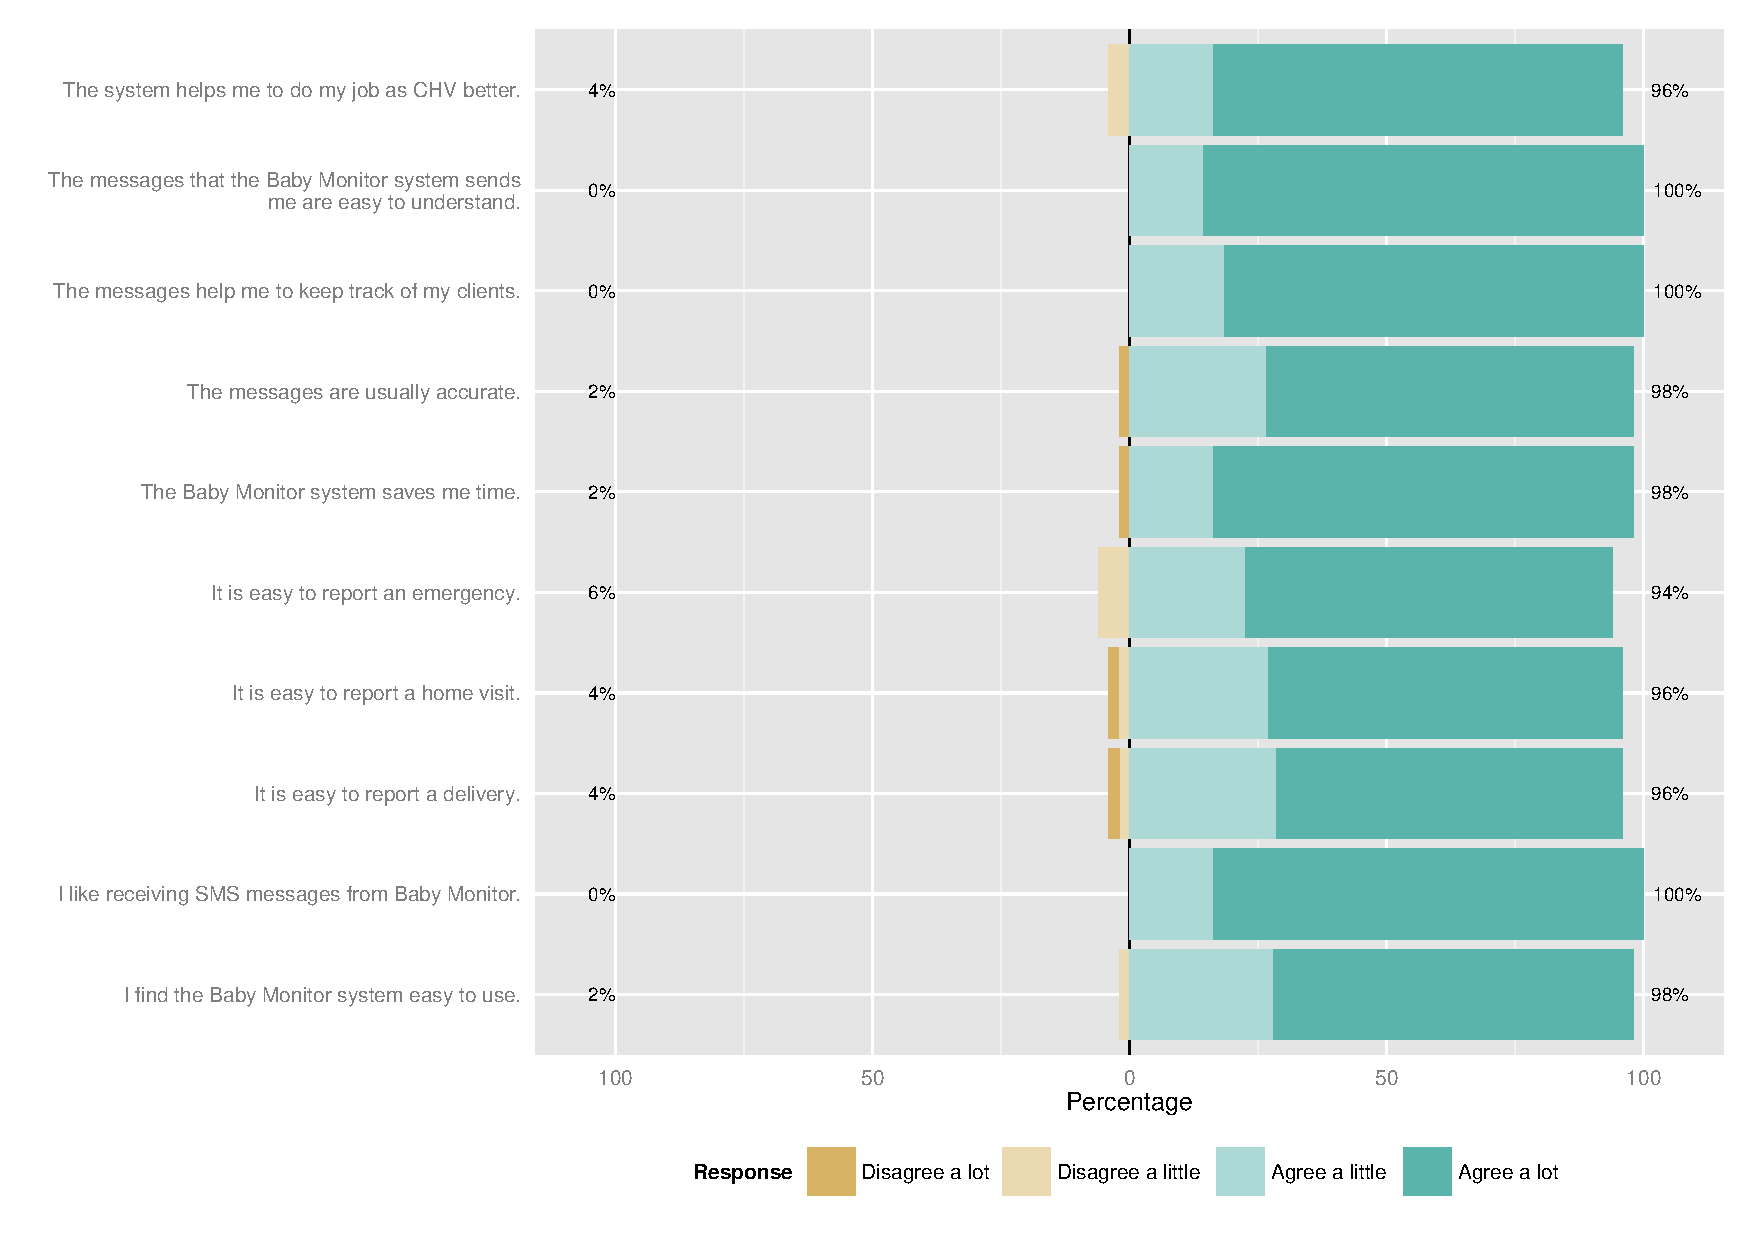
\includegraphics[height=4.5in]{usability-bar-316}
	\end{center}
	\caption[Usability survey results]{CHVs generally found the service to be usable. The SMS messages sent by the system were among the highest rated features of the system. Overall, 94\% of respondents believed that the system helped them do their jobs as CHVs better than before.}
	\label{fig:barchart}
\end{figure}


\section{Discussion}

\subsection{Principal Results}
\paragraph{The Hear phase revealed three general areas in which the CHVs were involved in maternal and child health care: home visits with pregnant women and new mothers, monitoring new deliveries in the community, and emergency care. Within each of these areas, three key themes emerged as priorities for the CHVs in designing a new patient management system: the need for fast, easy, data reporting methods, improved communication between CHVs and the clinic regarding referrals, and the need for an effective, reliable way to report and respond to obstetric emergencies. These themes led to the inclusion of five key design features that complemented the daily tasks of CHVs in the study catchment area, which are outlined as follows:}
\begin{enumerate}
	\item Reporting of home visits through IVR
	\item Notification of referred patients visiting the clinic through text message
	\item Reporting of deliveries through IVR
	\item Notification of patients delivering at the clinic through text message
	\item Reporting of emergencies directly to the clinic through IVR
\end{enumerate}

\paragraph{Mock testing of these features during the Create phase revealed enthusiasm and satisfaction with the service, but concerns were raised regarding the ability for CHVs to flash the Baby Monitor phone number should they run out of phone credit. This issue was addressed by including m-Pesa payments, which can be transferred directly into phone credit, for CHVs participating in the study.}

\paragraph{CHVs generally found the system to be usable. The text messages notifying CHVs of patient visits and deliveries were among the highest rated features of the system. }\todo{This section to be updated once results are complete. - A}

\subsection{Limitations}
This study piloted an intervention that was previously untested in this target population. Thus, the scope of the study was limited to a single clinic and a small, convenience sample of CHVs working in the clinic's catchment area. Participants for focus groups were selected based on English comprehension and demonstrated interest in the study, and thus may not generally represent the perspectives or viewpoints of all other CHVs within the health system. Due to time contraints, only one cycle of the Hear and Create phases were completed; in future iterations, additional cycles of prototyping and mock testing would have been conducted in order to refine and create additional features for the system.  

\subsection{Comparison with Prior Work}

- MoTECH program: IVR/texts in Ghana for midwives
- Believe that this has potential to improve community-based maternal and child health care

\subsection{Conclusions}}

%-----------------------------------------------------------------------------%
% Chapter 3: Reflection
%-----------------------------------------------------------------------------%
\chapter{Chapter Three}

%This chapter will  summarize the overall project, with a focus on lessons learned, implications for future research and intervention, and limitations. It can, but does not have to, include a more personal reflection on the research process. 

\section{Lessons Learned}
\begin{description}
	\item[Translation of messages may be best completed orally.] \hfill \\
	The process of translating all voice and text messages into the local dialect of Swahili proved to be much more challenging than expected. Since discussions with the CHVs and nurses during the Hear and Create phase were all conducted in English, it was difficult to translate into Swahili while maintaining the integrity of the original content. A woman local to the Ndivisi division was recruited to translate and later record the voice messages, as she was familiar with traditional Kenyan Swahili and Luhya, the language spoken by the native tribes in the region. However, the language spoken in Ndivisi division and surrounding areas blended elements of both languages; thus, it was difficult to come to a consensus on which translations would be understood by the majority of people living in the region. Additionally, many of the voice and text messages involved vocabulary and phrasing with which the translator was not familiar. Ultimately, the research team opted to use Google Translate as a tool for creating initial translations. These translations were then read to the translator, who then provided corrections orally. Although this process was extremely time-intensive, it yielded voice and text message prompts that were rated to be easy to understand and accurate by 100\% CHVs who participated in the usability survey at the conclusion of the study. 

	\item[Voice message quality is crucial to the success of an IVR system.] \hfill \\
	Prior to the mock testing session of the service during the Create phase, the research team recorded the complete set of audio messages at a residence in the nearby town of Webuye. At first, the team was not concerned about background noise from cows, chickens, or neighbors affecting the recording, as it would give the voice messages the feel of speaking to someone else in their home environment over the phone. However, testing of the voice messages during the mock session revealed that the audio messages suffered in quality when heard through users' phones. Numerous attempts were made to create quiet recording environments, free of animal or human sounds, but this proved to be impossible. Eventually, the research team discovered a recording studio in Eldoret town and opted to complete the recordings there. While studio-quality recordings came at a much higher price than originally intended, CHVs who responded to the usability survey believed that the voice messages were easy to understand and navigate. 

	\item[Expect mobile network variability.] \hfill \\
	Mobile network coverage in the study catchment area was extremely variable. At times, service would be at full strength, while at others, poor coverage made it impossible to complete calls. Given that the study site was in a very remote and rural region, this poor network coverage was not surprising. However, inconsistent mobile network signal did have an impact on results of the study, specifically when compiling data on usage of the system over time. A large percentage of calls initiated by CHVs were dropped in progress, either due to users hanging up early or due to poor network coverage. While user error may have accounted for some of the dropped calls, the quality of network coverage is likely to have caused problems for users trying to access the system. Unfortunately, there was no possible way for the research team to address this issue during the study.
\end{description}


\section{Limitations}
This study piloted an intervention that was previously untested in this target population. Thus, the scope of the study was limited to a single clinic and a small, convenience sample of CHVs working in the clinic's catchment area. Participants for focus groups were selected based on English comprehension and demonstrated interest in the study, and thus may not generally represent the perspectives or viewpoints of all other CHVs within the health system. Due to time contraints, only one cycle of the Hear and Create phases were completed; in future iterations, additional cycles of prototyping and mock testing would have been conducted in order to refine and create additional features for the system.  

\section{Implications for Future Research}
Future studies can build upon these findings by expanding the scope of the study beyond one study clinic and its corresponding two community units. Additional focus groups from the CHV and nurse population would also contribute to a more robust exploration of the flow of information and people with respect to maternal and child healthcare at the community level in this region. From a design perspective, upcoming versions of the system will also aim to further integrate the Baby Monitor screening service with the patient management component, so as to alert CHVs and suggest steps for follow up when a woman presents with concerning screening results. This will enable CHVs to identify high-risk patients and to adjust their approach in visiting and caring for them at the community level. Future iterations of the intervention will also evaluate additional features that were suggested by CHVs during the mock testing sessions in the Create phase, such as text message reminders for CHVs about upcoming home visits and expected delivery dates of women enrolled with the Baby Monitor system from their village. 


\section{Conclusions}
}


%-----------------------------------------------------------------------------%
% Appendices
%-----------------------------------------------------------------------------%
\appendix
\chapter{Usability Survey }


\begin{table}[htp]
  \centering
  \caption{Modified version of the Health IT Usability Evaluation Scale developed by \cite{Yen2010}.}
    \begin{tabular}{ll}
    \toprule
    \textbf{Concept} & \textbf{Item} \\
    \midrule
    \textit{Perceived Ease of Use} &  \\
    \textit{} & 1. I find the Baby Monitor system easy to use.  \\
    \textit{} & 2. It is easy to report a home visit. \\
    \textit{} & 3. It is easy to report a delivery.  \\
    \textit{} & 4. It is easy to report an emergency.  \\
    \textit{Perceived Usefulness} &  \\
    \textit{} & 5. I like receiving SMS messages from Baby Monitor.  \\
    \textit{} & 8. The messages help me keep track of my clients.  \\
    \textit{} & 9. The Baby Monitor system saves me time.  \\
    \textit{User Control} &  \\
    \textit{} & 6. The messages that the Baby Monitor sends me are easy to understand.  \\
    \textit{} & 7. The messages are usually accurate.  \\
    \textit{Quality of Work Life} & \textbf{} \\
          & 10. The system helps me to do my job as a CHV better.  \\
    \bottomrule
    \end{tabular}%
  \label{tab:usabilitysurvey}%
\end{table}%


}

%-----------------------------------------------------------------------------%
% References
%-----------------------------------------------------------------------------%
\bibliographystyle{./Bibliography/apa} %Formats bibliography
\cleardoublepage
\normalbaselines %Fixes spacing of bibliography
\addcontentsline{toc}{chapter}{References} %adds References to your table of contents
\bibliography{./Bibliography/BabyMonitor} %your references file - change the path if needed



% temp
\listoftodos
































\end{document}
